\chapter{Literature review}

\section{Decision-making}

\todo{Differentiate between sequential and non-sequential decisions?}

\Gls{decision-making} is one of the main aspects of cognition. It is studied from different perspectives by many scientific disciplines, from psychology and neurosocience to artificial intelligence and economy.

\subsection{The sequential nature of decisions}

Everyday, humans and non-humans make thousands of \glspl{decision}, each of them leading to a \gls{choice}. Many of those decisions are trivial (for example, choosing which socks to wear when dressing up). Others imply higher stakes (for example, deciding to embark oneself on a PhD).

Several traits of decisions illustrate their sequential nature \cite{forstmannSequentialSamplingModels2016}. All decisions are made under a form of time pressure: one simply cannot take hours to ponder over his or her socks collection, or wait indefinitely before accepting a PhD offering. A decision takes place at the end of a deliberation phase, where available information is acquired and processed. Many decisions are based on information that unfolds over time (for example, tasting wine before recognizing its grape variety). Even if all informative is immediately available (for example, a chessboard observed by a player before choosing his or her next move), it generally has to be treated sequentially, reflecting the frequent inability of the decision maker's cognitive system to process all information simultaneously.

A decision can be formalized as the mapping from a stimulus to a response. Time between stimulus and response execution is called \acrfull{rt} \cite{forstmannSequentialSamplingModels2016}, \cite{myersPracticalIntroductionUsing2022}.

$$RT = T_e+T_d+T_r$$

$T_{er}= T_e+T_r$ is called \textbf{non-decision time}.

\begin{figure}[ht]
    \centering
    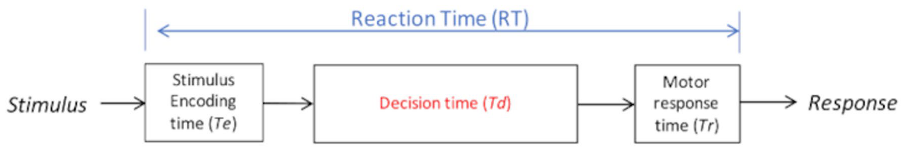
\includegraphics[width=\textwidth]{myersPracticalIntroductionUsing2022_1.png}
    \caption[Schematc of a decision]{Total \acrshort{rt} on each trial is assumed to reflect the time required to encode the stimulus ($Te$), the time to make a decision ($Td$), and the time to execute the selected motor response ($Tr$). The encoding and motor response time are typically combined into a single parameter, $Ter$, representing non-decision time. Adapted from \cite{myersPracticalIntroductionUsing2022}}
\end{figure}

\subsection{Decision types}

\todo{Decision types}

\subsection{The speed-accuracy tradeoff}

For decisions whose outcome can be evaluated (for example, recognizing a song based on its first notes), the balance between response time and accuracy is called the \acrfull{sat}. This ubiquitous aspect of decision-making has long been a phenomenon of interest in behavioral science \cite{heitzSpeedaccuracyTradeoffHistory2014}.

The \acrshort{sat} is at least partially under the decision-maker's control: a faster decisions cab ne taken at the expense of an higher error rate, and vice-versa \cite{ratcliffDiffusionDecisionModel2016}. As such, models of the decision must not only consider accuracy and speed, but the interaction between them \cite{myersPracticalIntroductionUsing2022}.

\subsection{Models of decision}

\subsubsection{Conceptual overview}

One approach to understanding decision-making is through computational models. Historically, most research has been focused on simple, repeatable problems involving decisions with one correct answer.

In this context, a decision can be thought of as a form of statistical inference \cite{goldNeuralBasisDecision2007}. A decision-maker must select among $K \in \mathbb{N^{+}}$ competing hypotheses denoted $h_k$, with $K \ge 2$ and $k \in [1,K]$. For example, a jury may have to rate each defendant on a scale of 1 (\textit{most certainly guilty}) to 5 (\textit{most certainly innocent}).

The probability $P(h_k)$, called \textit{prior}, refers to the probability that $h_k$ is true before obtaining any information about it. In the courtroom analogy, these priors correspond to prejudices that can bias jurors’ judgments.

Deciions are informed by data, called evidence and denoted $e$. Each evidence bears on a particular hypothesis $h_k$. For example, a DNA sample collection can be used as evidence for either supporting or opposing the hypothesis that a person was present at a crime scene. Thus evidence can be interpreted in the context of conditional probabilities such as $P(e|h_k)$, the likelihood function describing the values that $e$ can attain when $h_k$ is true.

Priors and evidence \todo{Add value?} are integrated into a conceptual entity called a \acrfull{dv}. In our example, the \acrshort{dv} correspond to the deliberation of the jury. A decision rule determines how the \acrshort{dv} is interpreted to commit to a particular alternative $H_k$ (the choice associated with hypothesis $h_k$). The rule causes the jury to declare, “we have a verdict.” In situations where the \acrshort{dv} can be expressed as a quantity, a simple rule is to place a criterion value on it: the decision is made if (or when) the \acrshort{dv} reaches this threshold.

\todo{Introduce the EAM family?}

\subsubsection{Signel Detection Theory}

\acrfull{sdt} is a framework for analysing \gls{decision-making} in the presence of \todo{Define uncertainty?} \gls{uncertainty}. Originally developped in the mid-20th century to assess how faithfully a radar operator was able to separate signal (enemy missiles or planes) from noise (random interferences or electronical artefacts), it has applications in many fields (psychology, diagnostics, quality control, etc) \cite{green1966signal}.

\acrshort{sdt} measures the ability of a decision-maker to discriminate two possible stimulus types \cite{stanislawCalculationSignalDetection1999}. A simple example of using \acrshort{sdt} in experimental psychology is when testing the ability of a subject to detect a short tone (signal) in a background of white noise. Another example could be a memory recognition test: assess stimuli items as already seen (signal) or new (noise).

\todo{Put this part (response matrix) sooner?} In a binary ("yes/no") task where signals were either present or absent in the stimuli, the responses given by the subject for each trial can be sorted un one of four categories (Table \ref{table:1}).

\begin{table}[h!]
    \centering
    \begin{tabular}{ ||c||c|c|| }
        \hline
        Signal  & Response: "absent"        & Response: "present" \\
        \hline\hline
        Absent  & Correct Rejections ($TN$) & False Alarms ($FP$) \\
        \hline
        Present & Misses ($FN$)             & Hits ($TP$)         \\
        \hline
    \end{tabular}
    \caption{Categorization of responses in a binary decision task.}
    \label{table:1}
\end{table}

The \textit{hit rate} (the probability of responding yes on signal trials), also called \acrfull{tpr}, and the \acrfull{fpr}, the probability of responding yes on noise trials, fully describe results.

$$\text{TPR} = \frac{TP}{TP + FN}$$

$$\text{FPR} = \frac{FP}{TN+FP}$$

\acrshort{sdt} represents a decision as a comparison between a \acrfull{dv}, directly derived from a single piece of evidence (stimulus), and a criterion (the threshold between the “noise” and “signal” responses) set by the decision-maker. This model can be applied to decision tasks in which a single stimulus is presented on each trial. Depending on the task, the \acrshort{dv} might be observable, or available only to the decision-maker. For example, the \acrshort{dv} may be the loudness experienced during each trial in an auditory perception study, or the feeling of familiarity associated with each stimulus item in a memory study.

However, factors both external (such as variations in stimulus strength) and internal (such as neural noise or limited resources) may affect the \acrshort{dv}. It will have a range of different values across signal trials and a range of different values across noise trials. The distribution of values realized by the \acrshort{dv} across signal trials is the \textit{signal distribution}, whereas the corresponding distribution for noise trials is the \textit{noise distribution}. These conditionalized distributions define the likelihoods $P(e|h_k)$ (value of $e$ in the presence/absence of signal). In the general case, the two distributions will overlap, reflecting the task difficulty (Figure \ref{figure:sdt}).

\begin{figure}[ht]
    \centering
    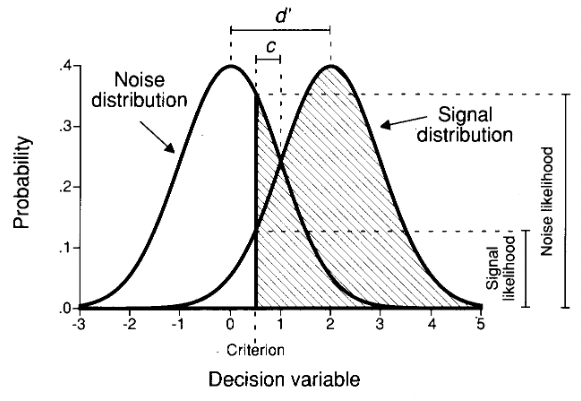
\includegraphics[scale=0.6]{stanislawCalculationSignalDetection1999_1.png}
    \caption[\acrlong{sdt}: graphical formalism]{\acrlong{sdt}: hypothetical probability density functions (likelihoods) for noise and signal distributions of the \acrlong{dv}. The \acrshort{dv} (measured in arbitrary units) has a mean of 0 and a standard deviation of 1 on noise trials. On signal trials, the mean is higher ($M = 2$), but the standard deviation is unchanged. A \textit{yes} response is made for trials in which the decision variable exceeds the criterion, located at $0.5$; these trials lie in the shaded region of the two distributions. The \acrlong{tpr} equals the proportion ofthe signal distribution that exceeds the criterion ($\acrshort{tpr} = 0.9332$). The \acrlong{fpr} equals the proportion of the noise distribution that exceeds the criterion ($\acrshort{fpr} = 0.3085$). Response bias can be quantified by either the likelihoods ratio $\beta$ at the criterion location ($\beta = \frac{0.1295}{0.3521} = 0.37$), or the distance $c$ between the criterion and the neutral point ($c = -0.5$). Both distributions are normal and of equal variance, so $d'$ is a bias-free measure of sensibility ($d'=2$). Adapted from \cite{myersPracticalIntroductionUsing2022}}
    \label{figure:sdt}
\end{figure}

\acrlong{sdt}'s main virtue is its ability to disentangle two factors in a decision process: the tendency towards responding \textit{yes} regarless of the stimulus, called \textit{bias}, and the ability to distinguish signal from noise, called \gls{sensitivity}. For example, industry quality-control inspectors often detect fewer faulty items as their work shift progresses. \Acrshort{sdt} demonstrated that this declining hit rate usually results from a change in response bias rather than a declining \gls{sensitivity} \todo{Citation too old}.

Bias is determined by the criterion location. A lower (liberal) criterion biases the decision-maker towards \textit{yes} responses, while a higher (conservative) value has the opposite effect. Bias can be quantified using either the ratio of the likelihoods for the two distributions at the criterion location (denoted $\beta$), or the distance between the criterion and the neutral point where distributions cross and neither response is favored, denoted $c$ and measured in standard deviation units.

\Gls{sensitivity} is determined by the degree of overlap between the noise and signal distributions. It is related to the distance between the means of the noise and signal distributions. One possible measure of \gls{sensitivity} is $d'$, which is the distance between the means in standard deviation units. Two assumptions must be met for $d'$ to be a bias-free measure of sensibility: the noise and signal distributions must be normal (Gaussian) and have the same variance (standard deviation). It can be obtained using the inverse cumulative distribution function, which computes the standard score (z-score) associated to a probability \cite{stanislawCalculationSignalDetection1999}.

Another possible measure of sensibility uses the \acrfull{roc} curve, which plots the \acrlong{tpr} as a function of the \acrlong{fpr} for all possible values of the decision criterion. Computing the \acrfull{auroc} is a non-parametric way to assess \gls{sensitivity} independently of bias that is free from the equal-variance Gaussian assumptions needed for $d'$ to be bias-free \cite{flemingHowMeasureMetacognition2014} (Figure \ref{figure:roc_curves}).

\begin{figure}[ht]
    \centering
    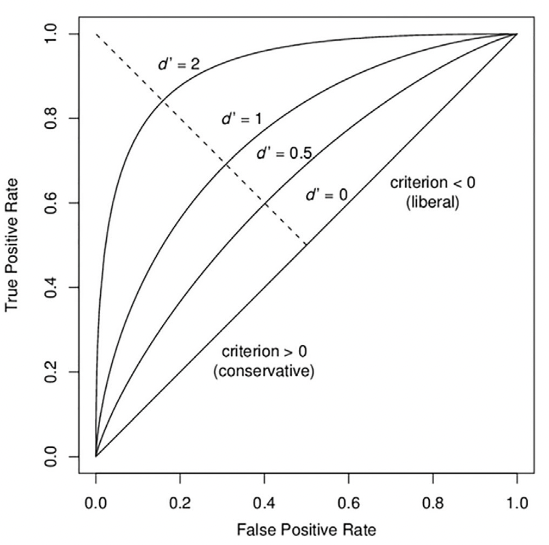
\includegraphics[scale=0.5]{michelConfidenceConsciousnessResearch2023_1.png}
    \caption[\acrlong{sdt}: \acrshort{roc} curves]{\acrlong{sdt}: \acrshort{roc} curves connecting locations with constant $d'$. The major diagonal is called the “chance line” since the \acrlong{tpr} and \acrlong{fpr} are equal, meaning that the subject is performing at chance level. A conservative criterion decreases both \acrshort{tpr} and \acrshort{fpr}, and a liberal criterion increases them. Using the \acrlong{auroc} is a way to assess \gls{sensitivity} independently of the response criterion. Adapted from \cite{michelConfidenceConsciousnessResearch2023}}
    \label{figure:roc_curves}
\end{figure}

\subsubsection{SPRT}

...

\section{Metacognition}

\section{Confidence}